\documentclass[12pt, a4paper]{article}

\usepackage[slovene, english]{babel}
\usepackage[utf8]{inputenc}
\usepackage{amsmath, amsfonts}
\usepackage{url}
\usepackage{graphicx}
%\usepackage{textpos}
\usepackage{wrapfig}
\usepackage{amsthm}
\usepackage{listings}
\usepackage{bm}
\usepackage{float}


%Tukaj lahko definiraš nova okolja in oznake
\newtheorem{izrek}{Izrek}
\newtheorem{trditev}{Trditev}
\newtheorem{lema}{Lema}
\newtheorem{definicija}{Definicija}
\newtheorem{pos}{Posledica}
\setlength\parindent{0pt}
%Za številske množice uporabi naslednje simole
\newcommand{\R}{\mathbb R}
\newcommand{\N}{\mathbb N}
\newcommand{\Z}{\mathbb Z}
\newcommand{\C}{\mathbb C}
\newcommand{\Q}{\mathbb Q}

\renewcommand{\mod}{\operatorname{mod}}
%Izpolni naslov in avtorje s svojimi podatki
\title{Seminarska naloga za Statistiko}
\author{Nejc Zajc}
\date{\today}

\begin{document}
\selectlanguage{slovene}
\maketitle

\section*{Metode dela}

Seminarsko nalogo sem rešil s programi v programskem jeziku \textit{Python}. Poleg osnovnih metod, ki jih jezik vsebuje, sem uporabil tudi pakete \textsc{math}, \textsc{random}, \textsc{numpy} (za delo z matrikami), \textsc{scipy.stats} (za dostop do gostot porazdelitev znanih slučajnih spremenljivk) in \textsc{matplotlib} (za risanje grafov).

%%%%%%%%%%%%%%%%%%%%%%%% ------------------------------------------------
% naloga 1

\section*{Naloga 1}
V tej nalogi me zanima ocena povprečnega števila otrok med družinami, ki živijo v mestu s $4$ mestnimi četrtmi. Z $\mu$ označim pričakovano vrednost tega števila. Zbrani podatki zajemajo podatke za $N = 43886$ družin, ki jim priredim zaporedne indekse od $0$ do $43885$.

\subsection*{Podnaloga a)}
V prvem delu z naslednjo kodo vzamem enostavni slučajni vzorec $n=400$ družin:
\begin{lstlisting}[language=Python]
izbrana_stevila = set()
while len(izbrana_stevila) < n:
    a = random.randint(0, N-1)
    izbrana_stevila.add(a)    
\end{lstlisting}
Število otrok na družino v celotni populaciji sedaj izračunam na podlagi podatkov za družine, ki so bile izbrane v vzorec. Za $i$-to izbrano družino, označim število otrok z $X_i$. Tako je povrečno število otrok v vzorcu izračunano po formuli
\[
\overline{X} = \frac{X_1 + \cdots + X_{n}}{n} = 1.0050.
\]
Standardna napaka je izračunana po formuli
\[
\widehat{SE}_+ = \left( \frac{N-n}{N}\frac{1}{n(n-1)}\sum_{i=1}^n (X_i - \overline{X})^2 \right)^{1/2} = 0.0575.
\]
Povedali smo, da velja $T = \frac{\overline{X} - \mu}{\widehat{SE}_+}\ \dot{\bm{\sim}}\ \text{Student}(n-1)$. Zato je ob stopnji tveganja $\alpha$ aproksimativni interval zaupanja za $\mu$ naslednji
\[
\overline{X} - F^{-1}_{\text{Student}(n-1)}\left(1-\frac{\alpha}{2}\right)\widehat{SE}_+ < \mu <
\overline{X} + F^{-1}_{\text{Student}(n-1)}\left(1-\frac{\alpha}{2}\right)\widehat{SE}_+.
\]
Ko vstavim izračunane vrednosti in določim $\alpha = 0.05$, dobim
\[
0.8920 < \mu < 1.1180.
\]

\subsection*{Podnaloga b)}
Tokrat sem podatke stratificiral glede na mestno četrt, v kateri družine stanujejo. Z naslednjo kodo sem najprej preštel število družin v posameznih četrtih - seznam $N_i$. Nato sem izračunal kakšne deleže populacije predstavljajo četrti - seznam $w_i$. Proporcionalno alokacijo sem določil tako, da sem glede na njihove necele dele, dve vrednosti $w_i * n$ zaokrožil navzdol, ostali pa navzgor. Tako sem dobil alokacijo - seznam $n_i$.
\begin{lstlisting}[language=Python]
cetrt = 4
N_i = [0, 0, 0, 0]
for j in podatki:
    N_i[j[4]-1] += 1
w_i = [N_i[i] / N for i in range(cetrt)]
n_i = [w_i[i] * n for i in range(cetrt)]
n_i = [int(n_i[0]), int(n_i[1]) + 1, 
	int(n_i[2]) + 1, int(n_i[3])]  
\end{lstlisting}
Proporcionalna alokacija populacije je sledeča:
\begin{align*}
n_1 = 92, & \quad & n_2 = 95, & \quad & n_3 = 123, & \quad & n_4 = 90.
\end{align*}
Nato sem izmed vseh družin v vzorec izbral naključne in njihova števila otrok označil z $X_{i, j}$, kjer je $i$ stratum oziroma četrt, kjer živijo, in $j$ njihov indeks znotraj stratuma.
\newpage
\begin{lstlisting}[language=Python]
strat_izbrane = [set() for _ in range(cetrt)]
konec = [False for _ in range(cetrt)]
while not all(konec):
    a = random.randint(0, N-1)
    a_cetrt = podatki[a][4]
    if not konec[a_cetrt - 1]:
        strat_izbrane[a_cetrt - 1].add(a)
        if len(strat_izbrane[a_cetrt - 1]) 
        	== n_i[a_cetrt - 1]:
           konec[a_cetrt - 1] = True
\end{lstlisting}
Za izračun intervala zaupanja sem nato za vsak stratum izračunal povprečje števila otrok
\[
\overline{X}_i = \frac{X_{i, 1} + \cdots + X_{i, n_i}}{n_i}
\]
in nepristransko cenilko za varianco tega povprečja
\[
\widehat{\sigma}_i^2 = \frac{1}{n_i-1} \sum_{j=1}^{n_i}\left( X_{i, j} - \overline{X}_i \right)^2.
\]
Te rezultate združim v izračunu povprečja števila otrok stratificiranega vzorca
\[
\overline{X} = w_1\overline{X}_1 + w_2\overline{X}_2 + w_3\overline{X}_3 + w_4\overline{X}_4 =  0.9223.
\]
Ocena skupne standardne napake je 
\[
\widehat{SE} = \left( \sum_{i = 1}^4 \frac{w_i^2 \widehat{\sigma}_i^2}{n_i} \right)^{1/2} =  0.0591.
\]
Pri stratificiranem vzorcu velja $T = \frac{\overline{X}-\mu}{\widehat{SE}}\ \dot{\bm{\sim}}\ \text{Student}(\nu)$, kjer je
\[
\nu = \frac{SE^4}{\sum_{i = 1}^4 \frac{w_i^4 \sigma_i^4}{n_i^2(n_i-1)}}.
\]
Na tem mestu vstavim v izraz za $\nu$ cenilke za standardno napako in za variance ter tako dobim cenilko $\widehat{\nu}$. Aproksimativni interval zaupanja za $\mu$ je pri stopnji tveganja $\alpha$ naslednji
\[
\overline{X} - F^{-1}_{\text{Student}(\widehat{\nu})}\left(1-\frac{\alpha}{2}\right)\widehat{SE} 
< \mu <
\overline{X} + F^{-1}_{\text{Student}(\widehat{\nu})}\left(1-\frac{\alpha}{2}\right)\widehat{SE}.
\]
Ko vstavim izračunane vrednosti in določim $\alpha = 0.05$, dobim
\[
0.8062 < \mu < 1.0384.
\]
\begin{figure}[h!]
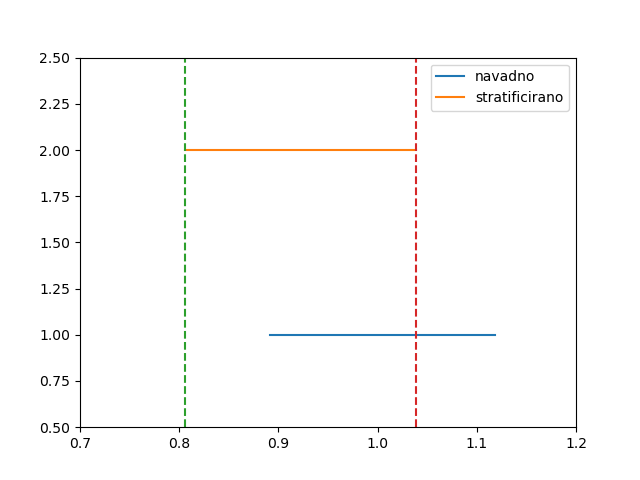
\includegraphics[width=\linewidth]{intervala_prva.png}
\centering
\caption{Primerjava intervalov zaupanja}
\end{figure}
Interval zaupanja, ki sem ga dobil s stratifikacijo je pomaknjen malo proti levi. Razlika med središči je majhna (relativno znaša dobrih $5\%$). Prav tako je njuna širina zelo podobna, interval zaupanja stratificiranega vzorca je malo večji (v tem primeru prb. za $2.5\%$ svoje širine). Tako lahko sklepam, da četrti v katerih živijo družine ne vplivajo močno na njihovo število otrok, kajti tudi če ne zagotovimo sorazmerne zastopanosti vseh četrti (kar je bistvo stratifikacije), razlika ni zelo velika.

%%%%%%%%%%%%%%%%%%%%%%%% ------------------------------------------------
% naloga 2
\section*{Naloga 2}
V nalogi 2 analiziram porazdelitev časovnih razmikov med zaznanimi fotoni.

\subsection*{Podnaloga a)}
Podatke preberem podobno kot v prvi nalogi in jih shranim kot števila $x_i$. Zbranih imam $n = 3935$ meritev. Največjo meritev si označim z $M$, najmanjšo pa z $m$. Za histogram najprej v skladu z modificiranim Freedman-Diaconisovim pravilom določim širino razredov $d$:
\begin{align*}
\text{IQR} = 87.60 & \quad &  d = \frac{2.6 \text{ IQR}}{\sqrt[3]{n}} = 14.43.
\end{align*}
Histogram narišem s pomočjo paketa \textsc{matplotlib}.
\begin{lstlisting}[language=Python]
import matplotlib.pyplot as plt
plt.hist(podatki, np.linspace(m, M, round((M-m)/d)))
\end{lstlisting}
\begin{figure}[h!]
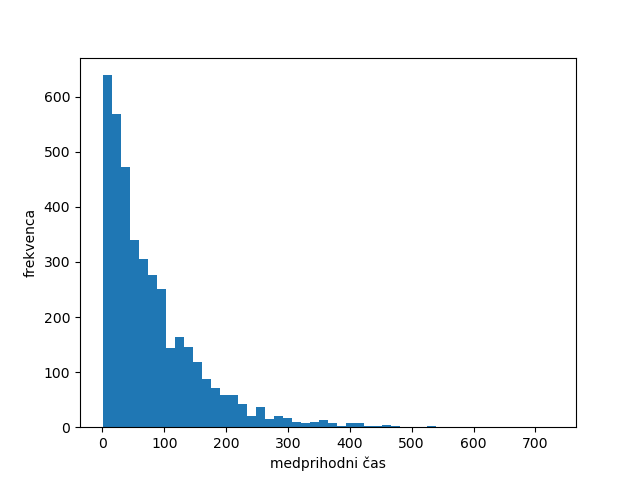
\includegraphics[width=\linewidth]{histogram_osnovno.png}
\centering
\caption{Histogram medprihodnih časov}
\end{figure}

Po primerjavi histograma z obliko gostote porazdelitve gama, se mi zdi model s to porazdelivijo verjeten, saj imata podobno obliko.

\subsection*{Podnaloga b)}
Porazdelitev gama, s parametroma $a$ in $\lambda$, ima gostoto $f_X(x) = \frac{\lambda^a}{\Gamma (a)}x^{a-1}e^{-\lambda x}$, kjer je $\Gamma$ funkcija gama.

Parametra najprej ocenim po metodi momentov. To smo naredili na vajah premeta Statistika (v št. letu 2020/2021) in dobili rezultat
\begin{align*}
\widehat{a}_{mm} = \frac{\overline{X}^2}{\overline{X^2} - \overline{X}^2}, & \quad &
\widehat{\lambda}_{mm} = \frac{\overline{X}}{\overline{X^2} - \overline{X}^2},
\end{align*}
kjer sta $\overline{X} = \frac{x_1 + \cdots + x_n}{n}$ in $\overline{X^2} = \frac{x_1^2 + \cdots + x_n^2}{n}$.

Zdaj ocenim parametra še po metodi največjega verjetja. Verjetje $L$ je produkt gostot za vse meritve $L(a, \lambda ; x_1, \ldots, x_n) = \prod_{i = 1}^n f_X(x_i)$. Za lažje računanje verjetje logaritmiram. Tako zdaj iščem maksimum funkcije
\begin{equation}
\label{eq:log_verj}
\ln(L) = l = na\ln(a) + (a-1)\sum_{i=1}^n\ln(x_i) - n\ln(\Gamma(a)) - \lambda(\sum_{i=1}^n x_i).
\end{equation}
Ko $l$ parcialno odvajam po $\lambda$ in enačim z $0$, dobim izražavo
\begin{equation}
\label{eq:lam}
\lambda = \frac{na}{\sum_{i=1}^n x_i}.
\end{equation}
To oceno zdaj vstavim v \eqref{eq:log_verj} in dobljeno funkcijo parcialno odvajam še po $a$. Med odvajanjem pridem do odvoda funkcije gama, ki se imenuje funkcija digama (z oznako $\psi$). Znan je približek te funkcije $\psi(x) \sim \ln (x) - \frac{1}{2x}$, ki ga uporabim, da lahko računam še naprej. Tako pridem do cenilke po metodi največjega verjetja
\[
\widehat{a}_{nv} = \frac{2}{\ln(\frac{\sum_{i=1}^n x_i}{n}) - \frac{\sum_{i=1}^n \ln(x_i)}{n}}.
\]
Cenilko za $\lambda$ sedaj dobim tako, da v izražavo \eqref{eq:lam} vstavim cenilko za $a$: $\widehat{\lambda}_{nv} = \frac{n \widehat{a}_{nv}}{\sum_{i=1}^n x_i}$.
Ko v vse cenilke vstavim meritve, dobim naslednje vrednosti:
\begin{align*}
\widehat{a}_{mm} = 1.0124, & \quad & \widehat{\lambda}_{mm} =  0.0127, \\
\widehat{a}_{nv} =  0.8917, & \quad & \widehat{\lambda}_{nv} =  0.0112.
\end{align*}
Vrednosti so podobne, opazim tudi, da je cenilka parametra $a$ v primeru metode momentov bližje 1, kar pomeni, da ta metoda porazdelitvi podatkov pripiše model, ki je bolj podoben eksponentni porazdelitvi, kot pa metoda največjega verjetja.

\newpage
\subsection*{Podnaloga c)}
Da sem lahko dorisal gostoti porazdelitev na isti graf kot histogram, sem moral linearno spremeniti ordinatno os grafa. Ta zdaj predstavlja relativno gostoto frekvenc. Nato na graf le dodam grafa gostot porazdelitve gama z izračunanimi cenilkami parametrov.

\begin{figure}[h]
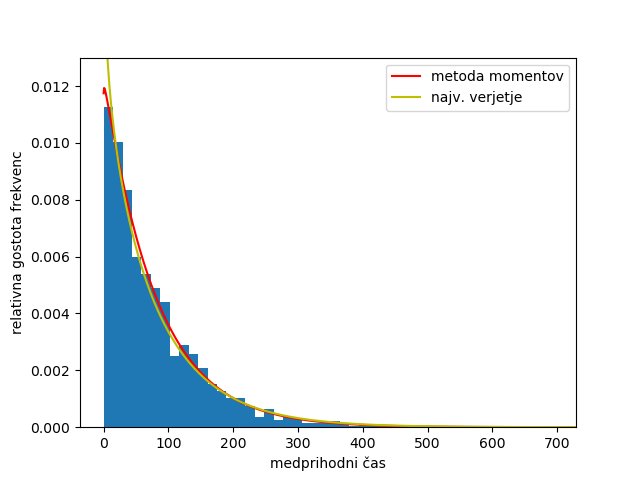
\includegraphics[width=\linewidth]{histogram_gostoti.png}
\centering
\caption{Histogram medprihodnih časov in gostoti porazdelitev}
\end{figure}

Histogram se prilega gostotama. Težko je reči, kateri bolje. Morda bi lahko rekel, da gostoti porazdelitve s cenilkama po metodi momentov, saj je ta gostota v osrednjem delu histograma malo višja.

\subsection*{Podnaloga d)}
Da lahko narišem histogram z logaritemsko lestvico na abscisni osi, moram najprej spremeniti širine območij, po katerih se zbirajo podatki za posamezen stolpec. Ta območja morajo biti zdaj eksponentno vedno večja, da bodo na logaritemski lestvici prikazana kot enako velika. Iz prejšnjega dela ohranim število stolpcev.

Območja stolpcev določim tako, da se začnejo tik pod najmanjšo vrednostjo podatkov (pri $0.10$) in končajo pri največji (pri $729.14$). Nato z ukazom paketa spremenim lestvico abscisne osi v logaritemsko in dobim željeni histogram.

\begin{figure}[h!]
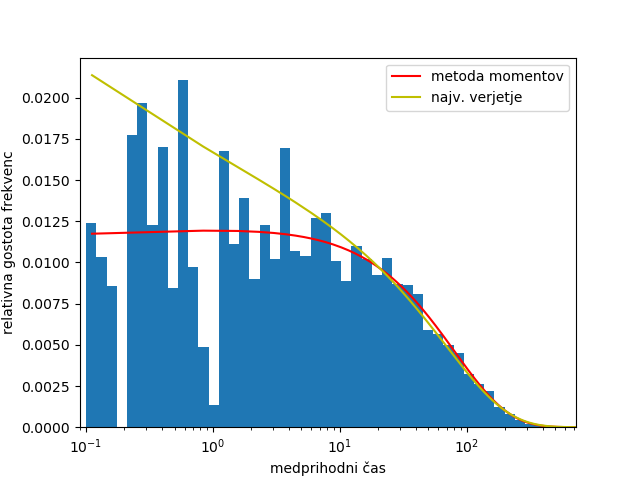
\includegraphics[width=\linewidth]{histogram_log.png}
\centering
\caption{Histogram in gostoti v logaritemski lestvici}
\end{figure}

Ta graf mi pove, da je v resnici precej natančnejša aproksimacija parametrov po metodi največjega verjetja, saj se pri majhnih časih veliko bolje ujema s podatki, kot pa aproksimacija po metodi momentov. Tako spremenim moje mnenje o tem, katera aproksimacija je boljša.

\subsection*{Podnaloga e)}
Poissonov model pravi, da so medprihodni časi porazdeljeni eksponentno. Izračunam še cenilko (po metodi največjega verjetja) za parameter $\lambda$ eksponentne porazdelitve za moje podatke. Ta cenilka je
\[
\widehat{\lambda} = \frac{n}{\sum_{i=1}^n x_i} = \frac{1}{\overline{X}} = 0.0125.
\]

\begin{figure}
    \centering
    \begin{minipage}{0.45\textwidth}
        \centering
        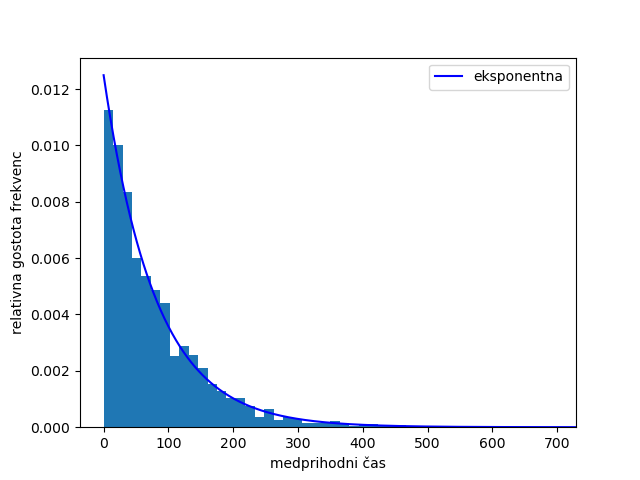
\includegraphics[width=\textwidth]{histogram_eksponentna.png} % first figure itself
        \caption{Histogram in gostota eks. por.}
    \end{minipage}\hfill
    \begin{minipage}{0.45\textwidth}
        \centering
        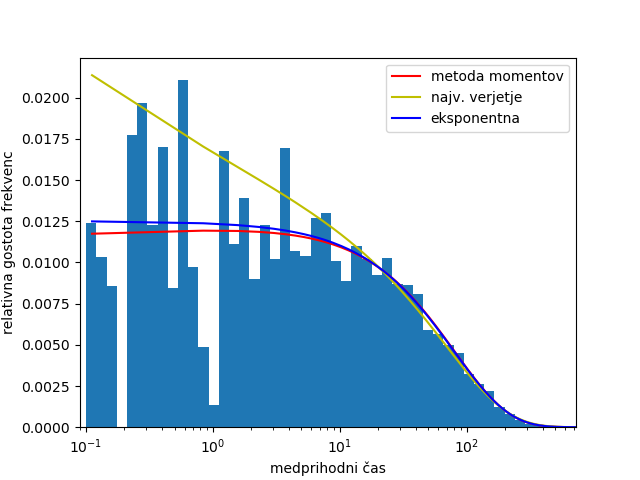
\includegraphics[width=\textwidth]{histogram_log_vse.png} % second figure itself
        \caption{Histogram in gostote v logaritemski lestvici}
    \end{minipage}
\end{figure}

Podatki se na navadnem histogramu tudi tokrat dobro prilegajo. Na logaritemskem pa se ne. Tako bi rekel, da Poissonov model ni najbolj točen, saj slabo oceni število zelo kratkih medprihodnih časov.


%%%%%%%%%%%%%%%%%%%%%%%% ------------------------------------------------
% naloga 3
\section*{Naloga 3}
V tej nalogi se ukvarjam z analizo vpliva dodajanja vitamina C na dolžino zob morskih prašičkov. Nalogo rešim z uporabo modela linearne regresije. Število podatkov v nalogi označim z $n=60$, med katerimi se $n_1=30$ morskim prašičkom vitamin dodaja neposredno, ostalim $n_2 = 30$ pa s pomarančnim sokom. Podatke si shranim v matrike s podobno kodo kot v nalogi 1. Pri tej nalogi si pri računanju z matrikami pomagam s paketom \textsc{numpy}.

\subsection*{Podnaloga a)}
Za začetek ne ločim med različnima načinoma dodajanja vitamina C in gledam le količino dodanega vitamina. V modelu linearne regresije je pojasnjevalna spremenljivka količina dodanega vitamina, odvisna spremenljivka pa dolžina zob morskega prašička.

V skladu z delom na predavanjih in vajah, označim z $Y_i$ dolžino zob $i$-tega morskega prašička, z $x_i$ pa količino vnešenega vitamina. Model je za vsak $i$ naslednji
\[
Y_i = a + bx_i + \varepsilon_i,
\]
kjer sta $a$ in $b$ iskana parametra regresije, $\varepsilon_i$ pa predstavlja napako oziroma šum. Predpostavim, da so $\varepsilon_i$ nekorelirane in da za vektor 
$\varepsilon =  \begin{bmatrix} \varepsilon_1 & \cdots & \varepsilon_n \end{bmatrix}^T$ velja $\varepsilon \sim N(0, \sigma^2 I_n)$.

Ko označim še $Y = \begin{bmatrix} Y_1 & \cdots & Y_n \end{bmatrix}^T$, 
$X = 
\begin{bmatrix}
1 & \cdots & 1 \\
x_1 & \cdots & x_n 
\end{bmatrix}^T$ in 
$\beta = \begin{bmatrix} a & b \end{bmatrix}^T$, dobim sistem
\[
Y = X \beta + \varepsilon.
\]

Na predavanjih smo povedali, da za konstanten vektor $c$ velja 
\[
T = 
\frac{c^T \widehat{\beta} - c^T \beta}{\widehat{\sigma}_+ \sqrt{c^T(X^T X )^{-1}c}}
\sim \text{Student}(n-p),
\]
kjer je $p$ število parametrov, oziroma dolžina vektorja $\beta$, $\widehat{\beta}$ cenilka po metodi najmanjših kvadratov za $\beta$ in $\widehat{\sigma}^2_+ = \frac{\text{RSS}}{n-p}$, če je RSS vsota kvadratov residualov $\text{RSS}= \lVert Y - X \widehat{\beta} \rVert $.

V nalogi preizkušam, ali dodajanje vitamina vpliva na rast zob, zato si postavim hipotezo, da dodajanje vitamina ne vpliva na rast in preverim, ali jo lahko zavrnem. Natančneje je moja hipoteza $H_0: b = 0$, torej da je regresijska premica vodoravna. Za vektor $c$ tako vzamem $c =  \begin{bmatrix} 0 & 1 \end{bmatrix}^T$, ob predpostavki $H_0$ pa velja $c^T \beta = 0$.

Ko sem si tako definiral vse potrebne pojme, sem najprej po metodi najmanjših kvadratov izračunal cenilko za $\beta$
\[
\widehat{\beta} = \left(X^T X\right)^{-1}X^T Y =
\begin{bmatrix} 7.4225 \\ 9.7636 \end{bmatrix}
\]
in nato še vrednosti v imenovalcu statistike $T$
\begin{align*}
\widehat{\sigma} = 4.6012 & \quad & \quad &
\sqrt{c^T(X^T X )^{-1}c} = 0.2070.
\end{align*}

Tako je vrednost statistike $T$, ko velja hipoteza $H_0$, enaka $T = 10.2501$. Ta račun sem izvedel z naslednjo kodo

\begin{lstlisting}[language=Python]
ocena_bete = np.matmul(
  np.linalg.inv(np.matmul(np.transpose(X), X)), 
  np.matmul(np.transpose(X), Y))

ocena_epsilon_vek = Y - np.matmul(X, ocena_bete)
ocena_sigma = math.sqrt(
  np.matmul(
    np.transpose(ocena_epsilon_vek), 
    ocena_epsilon_vek) / (n-p))

koren = np.matmul(
  np.transpose(c), 
  np.matmul(
    np.linalg.inv(np.matmul(np.transpose(X), X)), 
    c))
koren = math.sqrt(koren)

vrednost_T = (np.matmul(np.transpose(c), ocena_bete)) 
  / (ocena_sigma * koren)
vrednost_T = vrednost_T[0][0]
\end{lstlisting}

Hipotezo $H_0$ lahko zavrnem, če leži vrednost statistike $T$ izven intervala zaupanja za porazdelitev slučajne spremenljivke $\text{Student}(n-p) = \text{Student}(58)$. Pri stopnjah tveganja $5\%$ in $1\%$ sta ta intevala zaupanja naslednja
\begin{align*}
\alpha = 0.05 &: \ (- 2.0017, 2.0017), \\
\alpha = 0.01 &: \ (-2.6633, 2.6633).
\end{align*}
Ker leži $T$ tudi izven intervala zaupanja za $1\%$ stopjno tveganja, lahko hipotezo $H_0$ zavrnem. Trditev, da dodajanje vitamina vpliva na rast zob sprejmem, kar je jasno razvidno tudi iz grafa.

\begin{figure}[H]
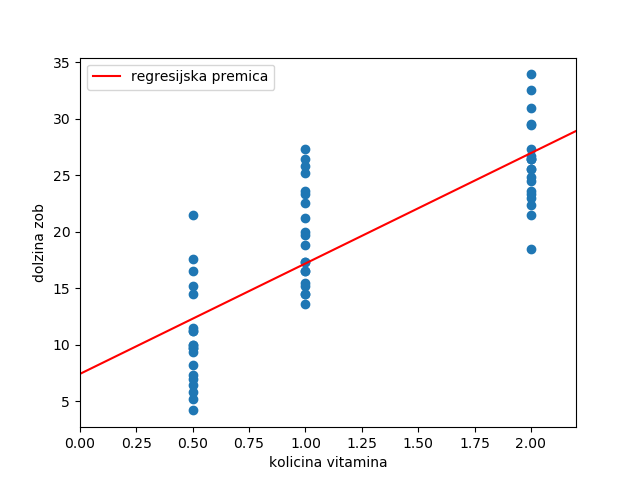
\includegraphics[width=\linewidth]{regresijska_premica.png}
\centering
\caption{Podatki in regresijska premica}
\end{figure}

\subsection*{Podnaloga b)}
Za konec moram preveriti še, kateri način je učinkovitejši in ugotoviti ali je razlika med načinoma statistično značilna. Učinkovitost načina dodajanja vitamina sem opredelil kot naklon regresijske premice tega načina. Za to sem se odločil, saj mi ta naklon pokaže dejansko povečanje dolžine zob pri večji količini vitamina, ne glede na morebitne razlike v začetni dolžini, ki se lahko kažejo v različnih začetnih vrednostih regresijskih premic.  

V tem primeru moram ločiti načina dodajanja. V podatkih naloge so najprej napisani primeri neposrednega vnosa, kot drugi pa primeri vnosa s sokom. Tako bo indeks $1$ predstavljal primer neposrednega vnosa, indeks $2$ pa primer soka. Matriki $X$ in $\beta$ se spremenita v naslednji
\begin{align*}
X =
\begin{bmatrix}
1 & x_1 & 0 & 0 \\
\vdots & \vdots & \vdots & \vdots \\
1 & x_{n_1} & 0 & 0 \\
0 & 0 & 1 & x_{n_1 + 1} \\
\vdots & \vdots & \vdots & \vdots \\
0 & 0 & 1 & x_n 
\end{bmatrix}
& \quad & \quad &
\beta = 
\begin{bmatrix}
a_1 \\
b_1 \\
a_2 \\
b_2 
\end{bmatrix}.
\end{align*}

Cenilka za vektor $\beta$ po metodi najmanjših kvadratov je (po enakem postopku kot v prvi podnalogi)
\[
\begin{bmatrix}
3.2950 \\
11.7157 \\
11.5500 \\
7.8114
\end{bmatrix}.
\]

V tem primeru je hipoteza, ki jo preverjam $H_0: b_1 = b_2$. Za vektor $c$ vzamem 
$c = \begin{bmatrix} 0 & 1 & 0 & -1 \end{bmatrix}^T$, saj tako $c^T \beta$ pove ravno razliko med naklonoma regresijskih premic, ki jo iščem. Ko hipoteza drži, je ta razlika enaka $0$. Enako kot v prvem delu zdaj izračunam statistiko $T$, ki ima ob predpostavki $H_0$ vrednost $T = 2.3094$.

Zaradi spremembe dolžine vektorja $\beta$, sta se spremenila tudi intervala zaupanja, ki sta sedaj
\begin{align*}
\alpha = 0.05 &: \ (- 2.0032, 2.0032), \\
\alpha = 0.01 &: \ (-2.6665, 2.6665).
\end{align*}

V primeru $5\%$ stopnje tveganja leži $T$ zunaj intervala zaupanja, zato hipotezo $H_0$ zavrnem. Ker je $T$ večji od zgornje meje intervala, to pomeni, da je vpliv direktnega vnosa vitamina dovolj močnejši od vnosa s pomarančnim sokom, da lahko hipotezo o enakem vplivu zavrnemo. Po drugi strani pa hipoteze pri $1\%$ stopnji tveganja ne morem zavrniti. Tudi tu dodam graf podatkov, tokrat so ločeni glede na način dodajanja vitamina.

\begin{figure}[h!]
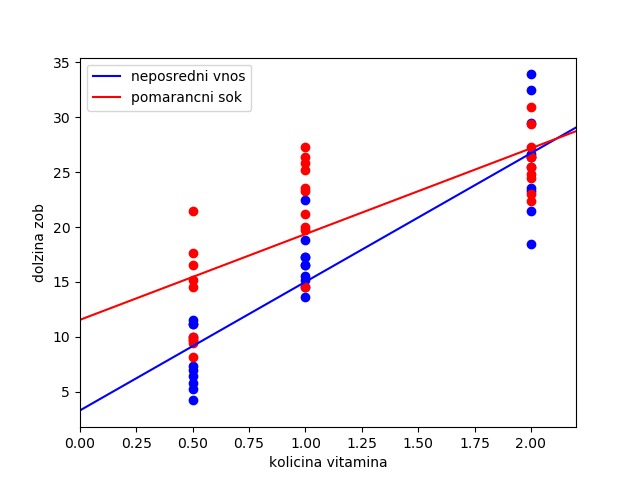
\includegraphics[width=\linewidth]{regresijska_premica_dve.png}
\centering
\caption{Ločeni podatki z regresijskima premicama}
\end{figure}


\end{document}